\section{Introduction}
\begin{multicols}{2}
En informatique, les Control Flow Graphs sont définis ainsi:
\begin{quotation}
    Un graphe de flot de contrôle (abrégé en GFC, control flow graph ou CFG en anglais) est une représentation sous forme de graphe de tous les chemins qui peuvent être suivis par un programme durant son exécution. \cite{wiki:Graphe_de_flot_de_controle}
\end{quotation}
A droite un exemple de CFG généré à partir du programme suivant:
\begin{lstlisting}[language=c]
    int main() {
        int a = 0;
        
        while(a < 1000) {
            if(a % 2 == 0) {
                a++;
            }
            else {
                a+=2;
            }
        }
    
        return 0;
    }
\end{lstlisting}
\begin{center}
    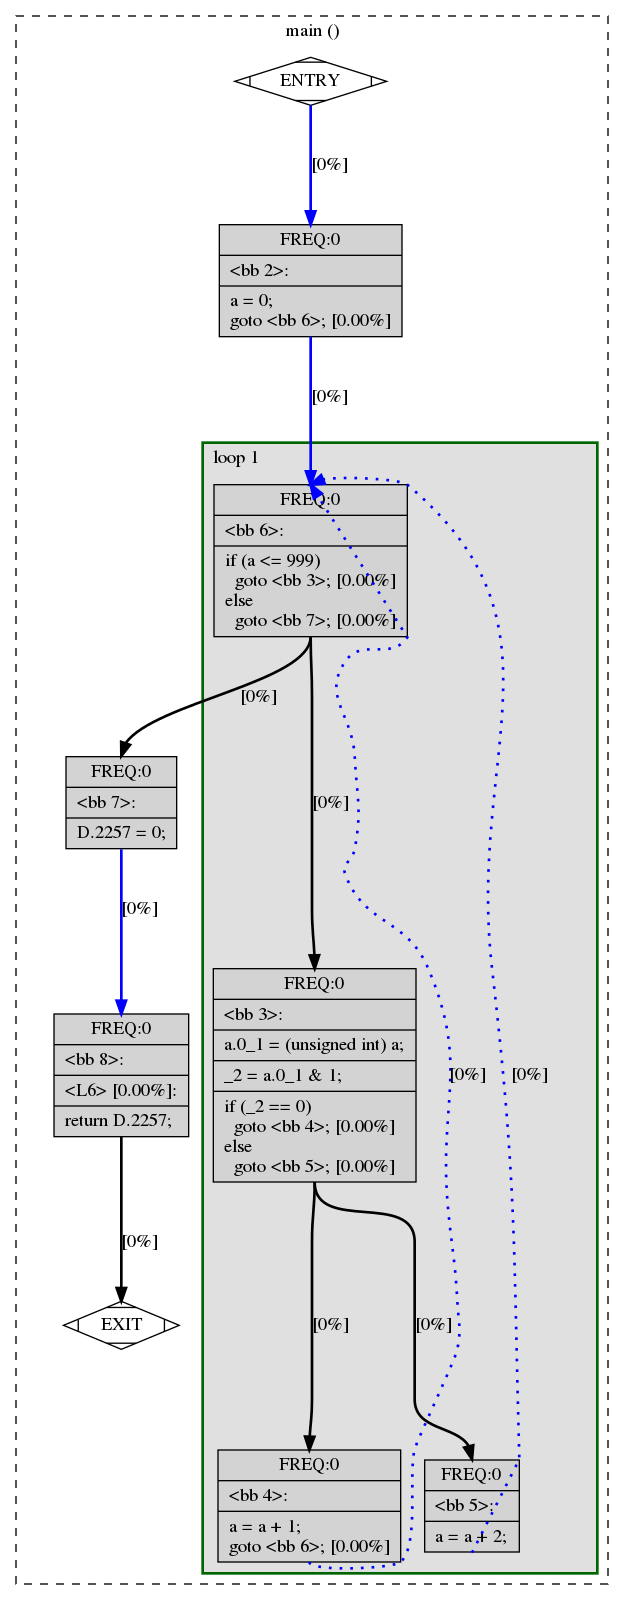
\includegraphics[scale=0.22]{images/graph.png}
    \captionof{figure}{Exemple CFG}
\end{center}
\end{multicols}
Comme l'exemple permet de le montrer, les graphes de flot de contrôle sont un excellent moyen de visualisation du code. Cependant sa véritable utilitée réside dans l'optimisation d'un code source.
\section{Nos recherches}

Afin d'étudier les Control Flow Graph, nous avons effectué un travail de recherche permettant de comprendre la modélisation des CFG, leur utilité et d'utiliser GCC pour générer et analyser des CFG. 

\subsection{Modélisation des CFG}
Nous allons dans un premier temps présenter la modélisation des CFG qui est déjà bien défini sur Wikipédia \cite{wiki:Graphe_de_flot_de_controle} mais approfondi dans la bible des compilateurs \cite{compilateurs}.

Les CFG font partis de la catégorie des graphes orientés. Cela signifie que ce sont des graphes dont les noeuds sont reliés par des arcs qui ont une direction. Les fonctions sont représentées par des sous-graphes disjoints les uns des autres.

Chaque noeud dans un CFG représente une portion de code, appelée \textbf{Bloc de base} dans laquelle il n'y a pas de saut ou de cible de saut. Un saut est défini par l'instruction \textit{goto xx} qui provient du langage assembleur et signifie \og saute à l'instruction xx \fg{}. L'entrée d'un bloc de base est la cible d'un saut, et la sortie est un saut.


Pour chaque fonction il existe toujours au moins deux blocs spéciaux. Le bloc \textit{Entry} qui caractérise l'entrée dans la fonction et donc le départ du flot, ainsi que le bloc \textit{Exit} qui caractérise la sortie de la fonction et la fin du flot.

Par construction le degré entrant et sortant d'un noeud, à part pour les blocs spéciaux définis ci-dessus, sont toujours supérieurs ou égaux à 1. En effet, si un bloc de base n'a pas de degré entrant, ce bloc n'est jamais exécuté et représente donc du code mort. Il peut alors être supprimé. De même, le seul bloc ayant un flot sortant nul est le bloc de sortie. 

Le code:
\begin{lstlisting}[language=c, numbers=left, xleftmargin=.35\textwidth]
    a = 0
    b = a + 70
    if b < 50
        print("Je ne vais pas afficher a")
        goto 7
    print(a)
    fin
\end{lstlisting}
se traduit en 4 blocs de base:
\begin{lstlisting}[language=c, xleftmargin=.26\textwidth]
    a = 0
    b = a + 70
    if b < 50

    print("Je ne vais pas afficher a")
    goto 7

    print(a)

    fin
\end{lstlisting}
et le graphe est représenté de la manière suivante:
\begin{center}
    \begin{tikzpicture}[
        node distance = 12mm and 6mm,
        box/.style = {rectangle, draw, fill=#1, 
                    minimum width=12mm, minimum height=7mm}
                    ]
        \node (n1) [box=white, align=justify] {a = 0\\b = a + 70\\if b < 50};
        \node (n2) [box=white, align=justify, below =of n1] {print("Je ne vais pas afficher a")\\goto 7};
        \node (n3) [box=white,below right=of n2] {print(a)};
        \node (n4) [box=white, below left=of n3] {fin};
        %
        \draw[->] (n1) to (n2);
        \draw[->, bend left] (n1) to (n3);
        \draw[->] (n2) to (n4);
        \draw[->] (n3) to (n4);
    \end{tikzpicture}
\end{center}

Les boucles introduisent un nouveau type d'arc: les \textit{arcs en arrière}. Ce sont des arcs spéciaux qui permettent de remonter à un arc déjà rencontré. En effet, un programme est exécuté ligne par ligne sauf lorsqu'une boucle fait explicitement remonter le programme à des instructions précédentes. 

Une boucle est constitué en en-tête d'un bloc \textbf{dominant} de la boucle qui représente sa condition et qui est la cible de l'arc en arrière. Ensuite ce bloc d'en-tête pointe vers la sortie de la boucle et vers le premier bloc de base de la boucle.

Voici un exemple:
\begin{lstlisting}[numbers=left, language=c, xleftmargin=.35\textwidth]
    a = -3
    while a > 0:
        a++
        goto 2
    print("sortie de boucle")
\end{lstlisting}

\begin{center}
    \begin{tikzpicture}[
        node distance = 12mm and 6mm,
        box/.style = {rectangle, draw, fill=#1, 
                    minimum width=12mm, minimum height=7mm}
                    ]
        \node (n1) [box=white, align=justify] {a = -3};
        \node (n2) [box=white, align=justify, below =of n1] {if a > 0};
        \node (n3) [box=white, align=justify, below =of n2] {a++\\goto 2};
        \node (n4) [box=white,below left=of n2] {print("sortie de boucle")};
        %
        \draw[->] (n1) to (n2);
        \draw[->] (n2) to (n3);
        \draw[->] (n2) to (n4);
        \draw[->, dashed, out = -40, in =40, looseness=2] (n3.south) to (n2.north);
    \end{tikzpicture}
\end{center}

Les CFG permettent également d'étudier le flot du programme c'est à dire de savoir de quelle manière l'exécution a tendance à s'effectuer. Si par exemple une condition a plus souvent une chance d'être vraie ou fausse, une boucle de se terminer ou non. Cela a des utilités pratiques pour le compilateur comme nous allons l'évoquer dans la prochaine section.

\subsection{Utilité des CFG}
Lors de la compilation, le code source subit plusieurs analyses et opérations \cite{compilateurs}:
\begin{itemize}
    \item \textbf{Le prétraitement:} En langage C par exemple, il existe des instructions pour le préprocesseur qui permettent de créer des macros et des compilations conditionnelles. Le prétraitement va se charger de remplacer les macros et de gérer la compilation condtionnelle.
    \item \textbf{L'analyse lexicale:} Le code est passé sous découpe laser afin de l'écrire sous forme de \textit{jetons} (ou \textit{tokens} en anglais) qui représentent les mots clef du langage, identifiants et symboles. 
    \item \textbf{L'analyse syntaxique:} Analyse de la suite des jetons afin de construire un arbre basé sur la grammaire du langage. Par exemple, une boucle contient toujours une condition.
    \item \textbf{L'analyse sémantique:} L'arbre précédemment construit reçoit des informations sémantiques. Durant cette phase, le compilateur vérifie le type des variables, construit la table des symboles (qui contient les identifiants des variables, leur \textit{scope}, ...).
    \item \textbf{Génération du code intermédiaire:} L'arbre est utilisé pour générer un code dit intermédiaire qui permet de réaliser des opérations plus aisées d'optimisation.
    \item \textbf{Optimisation du code intermédiaire:} Le code intermédiaire est optimisée afin de soit modifier le code pour le rendre plus efficace (exemple: suppression de variables inutiles par propragation de constante), ou supprimer du code mort détecté.
    \item \textbf{Génération du code:} Dernière étape durant laquelle, l'exécutable est créé.
\end{itemize}
Il est à noter que ces phases ne sont ni nécessairement linéaires, ni uniques. Le compilateur effectue des opérations parallèles entre différentes portions du code et des passes afin d'optimiser plusieurs fois le code généré.

Les CFG dans ces étapes d'optimisation servent à plusieurs choses. Tout d'abord, détecter du code mort car comme il a été dit en introduction, si un bloc de base n'a pas de degré entrant, alors il n'est jamais exécuté.

De plus, il est parfois utile de savoir quelle est la probabilité qu'un code soit exécuté afin que le compilateur privilégie une exécution plus rapide d'une branche plutôt qu'une autre. La documentation GCC évoque plus en détail cette étape \cite{gcc:cfg}.

Cependant, les CFG ne sont pas seulement utiles pour le compilateur, mais pour de nombreux analyseurs statiques. Il permet de connaitre l'ordre d'exécution d'un programme par sa construction en arbre, d'étudier si un programme / une fonction contient des boucles, la résilience d'un programme... Beaucoup d'analyse basée sur la théorie des graphes peuvent être effectués afin d'étudier la structure du code source à partir de sa représentation en graphe.

\subsection{Outil de GCC}
Afin de nous permettre d'étudier et de comprendre les CFG, nous avions besoin d'avoir un outil permettant de les générer. GCC via sa palette d'options de compilation nous a fourni cet outil. Par exemple via GCC\footnote{Commande Bash utilisée: \textbf{gcc -fdump-tree-all-graph <target.c>}}, le code et son graphe ci-dessous:
\begin{multicols}{2}
\lstinputlisting[language=c]{code/code.c}
\begin{center}
    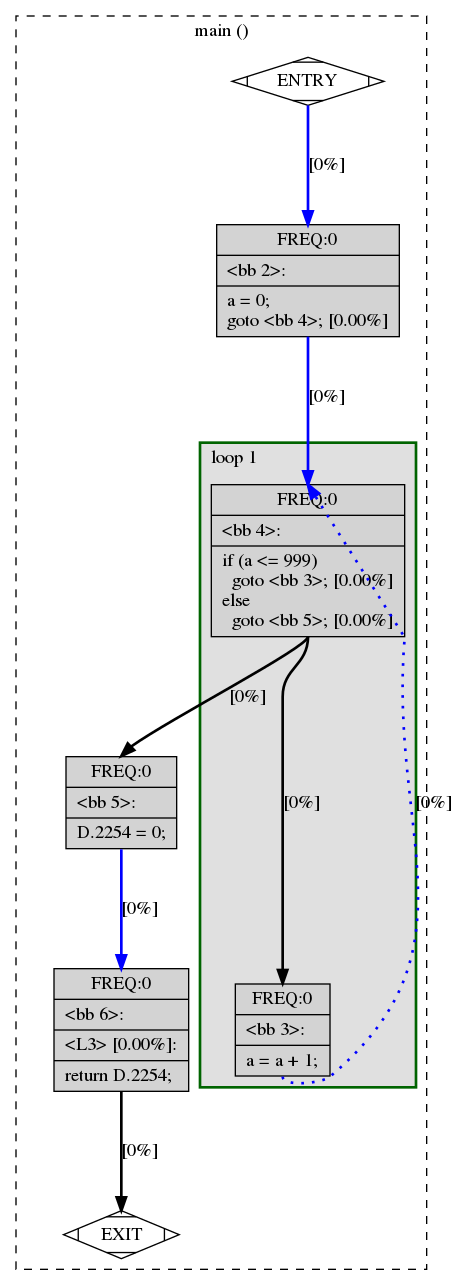
\includegraphics[scale=0.32]{images/graph2.png}
\end{center}
\end{multicols}
\section{Implémentation}
Dans le cadre de notre étude des CFG, nous avons réalisé deux scripts différents via l'utilisation de python et de différentes librairies.

Comme nous avons pu le voir, grâce à GCC, nous avons pu générer des CFG. Pour pouvoir avoir une représentation adéquate, GCC propose un fichier de sortie au format \textit{.dot}\footnote{Le langage DOT est un langage de description de graphe dans un format texte.}.
\subsection{Notre script de modifications des CFG}
De base, lorsqu'un CFG est généré, les fonctions sont séparées dans des sous graphes distincts. Cela est intéressant car il est alors possible d'analyser chacune des fonctions séparémment, ce qui est en générale l'intérêt d'une fonction, encapsuler du code.

Cependant, l'intérêt d'un CFG, c'est aussi de savoir comment le flot traverse le programme. Or, il peut-être intéressant de voir le flot entre deux fonctions. Nous avons donc développé un script permettant de raccorder deux fonctions lorsque celles-ci sont situées dans le même fichier.

Prenons l'exemple du code source suivant:
\lstinputlisting[language=c, xleftmargin=.35\textwidth]{code/cfg_avant.c}

\pagebreak
Le CFG fabriqué à partir de ce code par GCC est ceci:
\begin{center}
    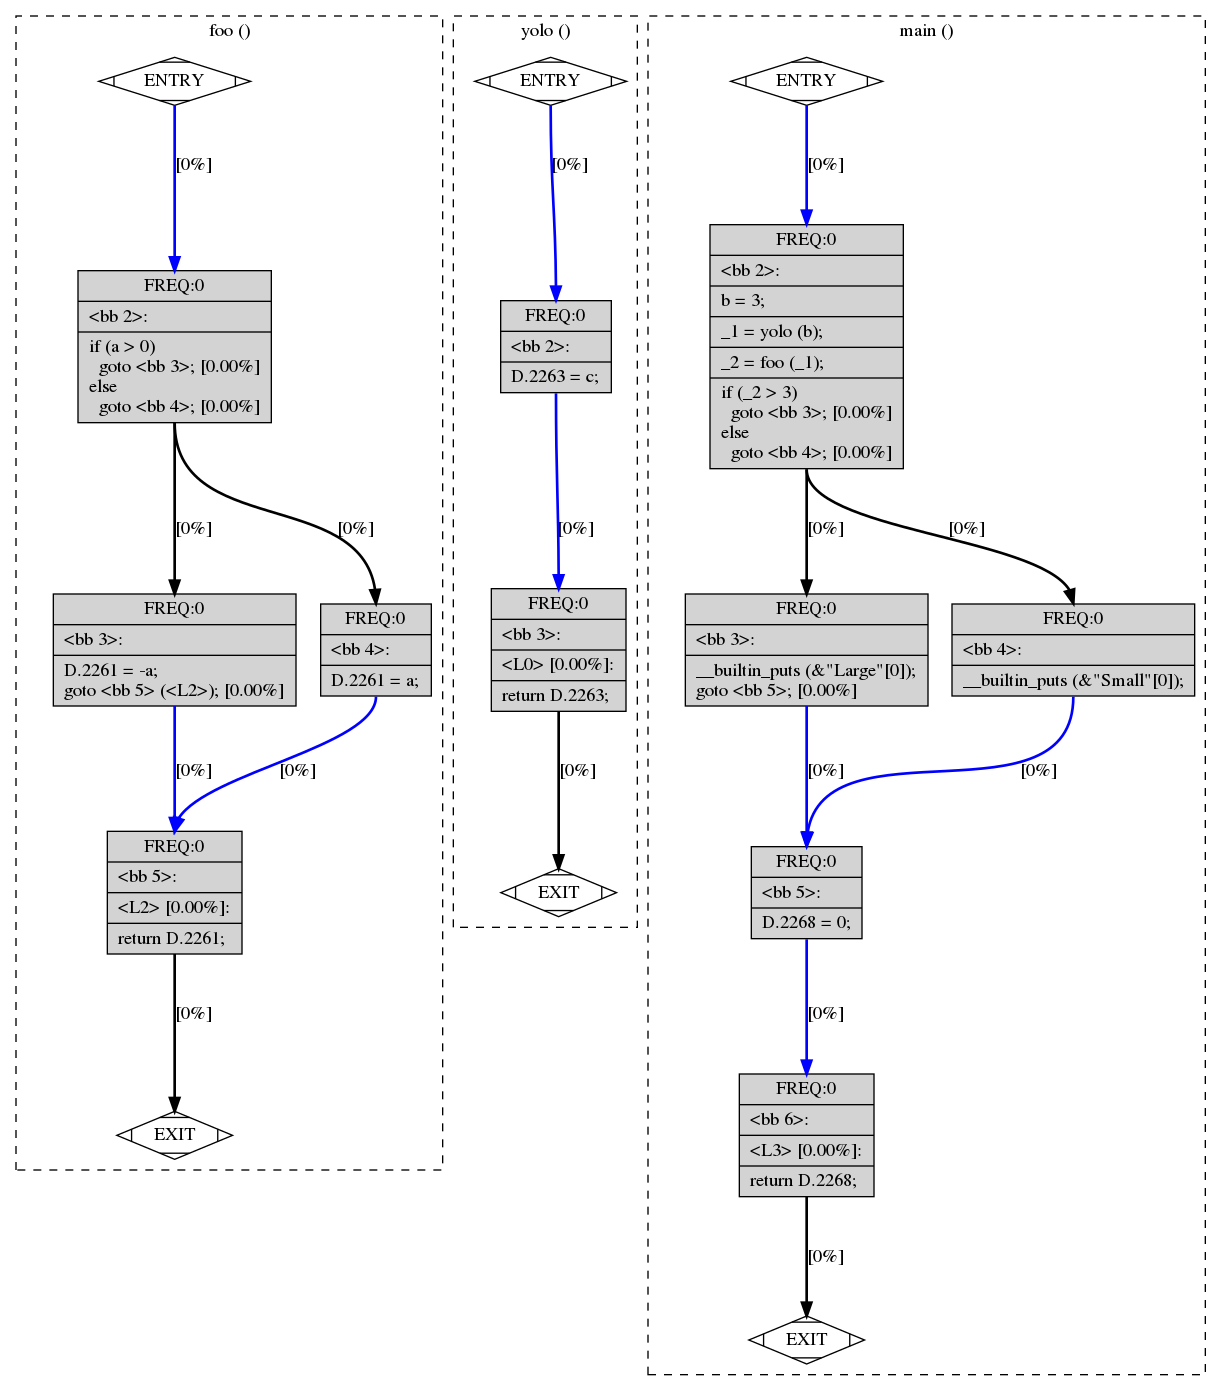
\includegraphics[scale=0.32]{images/cfg_avant.png}
\end{center}
Comme il est possible de le constater dans le code et le CFG, les appels à fonction sont identifiables dans ce programme et après passage du fichier dot représentant ce graphe dans notre script, voici le nouveau CFG que nous avons obtenu:
\begin{center}
    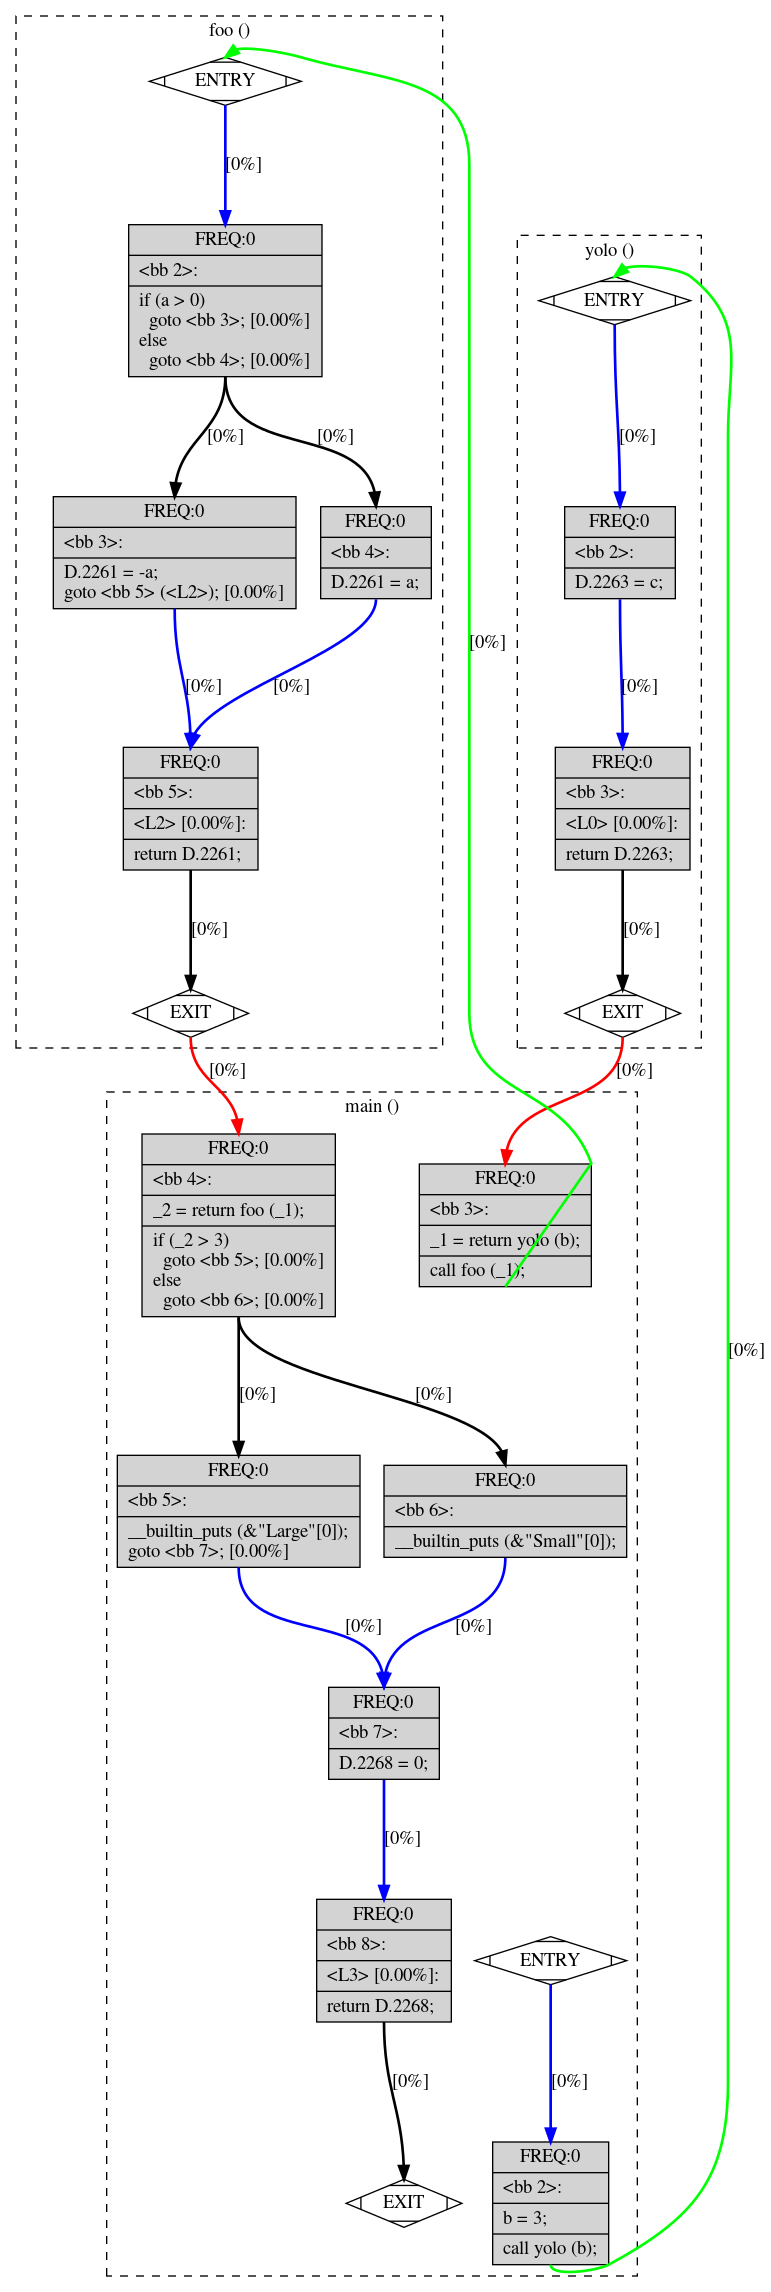
\includegraphics[scale=0.26]{images/cfg_apres.png}
\end{center}
Pour ce faire, nous avons utilisé une librairie appelée \textit{pydot}\footnote{Pydot est une librairie pouvant parser du code DOT généré par la librairie GraphViz (utilisée par GCC pour générer des CFG).} qui nous a permis de parser les fichiers DOT et de les modifier par le langage de programmation Python.

Nous avons décidé que les blocs de base spéciaux \textit{Entry} et \textit{Exit}, seront désormais des blocs normaux avec un flot entrant et sortant, sauf pour l'entrée et la sortie du programme. Les appels à fonctions sont désormais considérés comme des sauts et la variable de retour est la cible du saut de la fin de fonction, ce qui permet de définir deux nouveaux blocs de base à partir d'un appel à fonction.

On remarque que le flot passe maintenant dans les fonctions ce qui permet de mieux les situer les unes par rapport aux autres. Cela permet notamment d'identifier du code mort ou non utile dans le fichier parsé. En effet, si on remarque qu'une fonction n'est pas atteinte, cela signifie que son code n'est jamais exécutée (par les fonctions présentes dans son fichier).

\subsection{Notre script d'analyse des CFG}
Nous avons développé un second script permettant d'analyser les CFG en utilisant encore une fois Python et une librairie nommée \textit{NetworkX}\footnote{NetworkX est une librairie permettant de modéliser, analyser la structure et la dynamique de graphe via un lot de fonctions implémentées.}. Notre script permet d'analyser différentes choses.

Il identifie quels sont les noeuds qui n'ont pas de degré entrant, ce qui signifie qu'il est capable de détecter du code mort au sens du fichier, c'est à dire, si une fonction n'est pas exécutée par une autre dans un fichier. Il peut également détecter si un graphe est acyclique, c'est à dire si une boucle est présente ou non dans un graphe.

Le script renvoie également le plus court et long chemin entre le début et la fin du graphe (donc du programme) ce qui permet d'étudier quelles sont les différentes étapes d'exécution qui entraine une durée plus ou moins importante du programme.

Il permet également d'étudier la connectivité qui représente le nombre de possibilité moyenne pour aller d'un noeud à un autre. Plus ce nombre est haut, plus il y a de conditions dans le programme.

Pour le CFG de la section précédente après traitement par notre script de modifications des appels à fonction, le script d'analyse renvoie les résultats suivants:
\begin{itemize}
    \item Il y a un noeud sans entrée dans la fonction main, ce qui correspond à l'entrée du programme.
    \item Les chemins plus long et court font 17 noeuds.
    \item Le graphe est acyclique.
    \item Le graphe a une connectivité de 1.19.
    \item Il n'y a pas de noeuds isolés.
\end{itemize}
Analysons maintenant le graphe généré par notre programme:
\lstinputlisting[language=c, xleftmargin=.35\textwidth]{code/fonction_inutile.c}

Le graphe est alors:
\begin{center}
    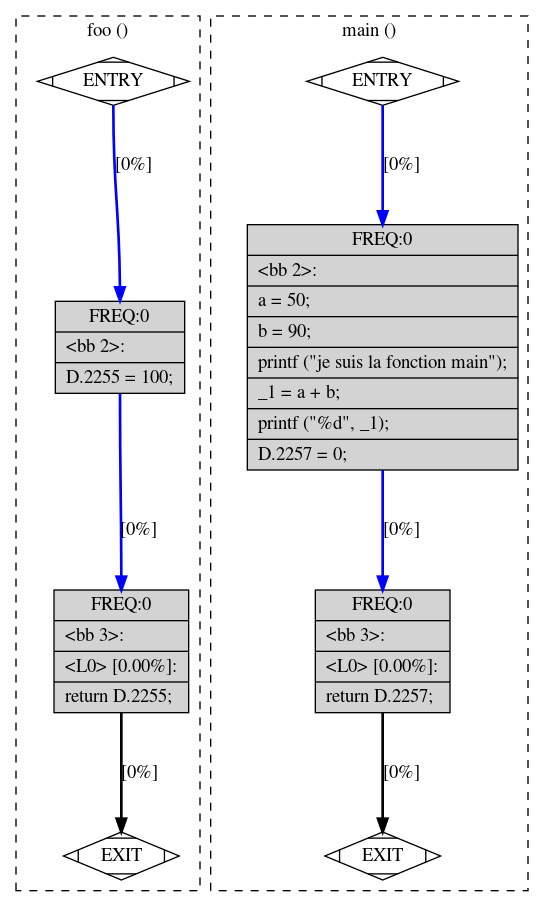
\includegraphics[scale=0.35]{images/fonction_inutile.png}
\end{center}

Notre script d'analyse renvoie ceci:
\begin{itemize}
    \item Il y a un noeud sans entrée dans la fonction foo
    \item Il y a un noeud sans entrée dans la fonction main
    \item Les chemins plus long et court font 4 noeuds.
    \item Le graphe est acyclique.
    \item Le graphe a une connectivité de 1.
    \item Il n'y a pas de noeuds isolés.
\end{itemize}
On remarque donc que notre programme a bien détecté qu'une fonction n'est jamais exécutée et donc qu'il y a du code mort. Le degré de connectivité a également baissé, ce qui est logique car il y a moins de chemins puisqu'il n'y a pas de conditions. Il n'y a toujours pas de noeuds isolés car la fonction foo contient plusieurs noeuds.